\chapter{Avaliação e Resultados} \label{chap:resultados}

A hipótese levantada no âmbito desta dissertação é que o uso de abstração em imagens que vão ser ser alvo de reconhecimento facial pode melhorar o processo de reconhecimento facial automático em imagens. Para a análise desta hipótese foi criado um sistema de reconhecimento facial automático em imagens, assim  como, escolhida uma biblioteca de imagens a analisar, tal como descrito no capítulo \ref{chap:visage}. Neste capítulo, é apresentada a avaliação efetuada ao sistema de reconhecimento facial criado, assim como, os diversos resultados obtidos. 

Em primeiro lugar, são apresentados os conjuntos de teste criados para efetuar a avaliação do sistema Visage, a partir da coleção LFW-a, na secção \ref{sec:conjuntos}.

Posteriormente são apresentadas as tarefas de pré-processamento a que as imagens de cada conjunto de teste foram sujeitas, em \ref{sec:experiencias}, das quais resultou a criação de um conjunto de galerias de imagens pré-processadas. 

Em terceiro lugar, são apresentadas as diversas avaliações efetuadas ao sistema, \textit{Closed-set Identification} e \textit{Image Retrieval}, as quais são apresentadas nas secções \ref{sec:avaliacao1} e \ref{sec:avaliacao2}, respectivamente. A primeira constitui uma medida padrão de avaliação do desempenho de sistemas de reconhecimento facial automático, a segunda, pretende analisar o desempenho do sistema de um ponto de vista mais próximo de um provável caso de uso, neste caso, \textit{Image Retrieval}. Para além destas duas avaliações, é ainda analisada a variação do desempenho do sistema nos diferentes conjuntos de teste utilizados, a qual se encontra reportada na secção \ref{sec:variacaodesempenho}.

Finalmente, em último lugar, é ainda apresentada uma análise aos resultados obtidos, na secção \ref{sec:discussao}.

\section{Conjuntos de Teste}  \label{sec:conjuntos}
O desempenho de sistemas de reconhecimento facial pode ser analisado através de diferentes perspetivas, tal como introduzido na secção \ref{sec:problema} desta dissertação. A biblioteca LFW foi criada com o propósito inicial da análise do sub-problema de reconhecimento facial \textit{pair matching}, no qual o sistema deve decidir se duas faces representam ou não o mesmo indivíduo. No entanto, as características desta biblioteca, nomeadamente no que diz respeito à existência da anotação textual das pessoas presentes em cada imagem, à existência de apenas uma pessoa representada (de forma relevante) em cada imagem e ainda da normalização do formato das imagens, permitem que esta biblioteca possa ser utilizada com um esforço reduzido para o analise dos restantes sub-problemas de reconhecimento facial automático. As avaliações de desempenho reportadas no âmbito desta dissertação nas secções \ref{sec:avaliacao1}, \ref{sec:avaliacao2} e \ref{sec:variacaodesempenho} não se enquadram no paradigma de \textit{pair matching}, para o qual a biblioteca LFW foi originalmente criada, pelo que se tornou necessário o desenvolvimento de novos conjuntos de teste, os quais passamos a apresentar de seguida.

Na avaliação de sistemas de reconhecimento facial automáticos designam-se de \textit{amostras biométricas} as capturas de características de uma pessoa que permitem efetuar o seu reconhecimento. Dependendo do sistema, as amostras biométricas podem ser apenas uma imagem, um conjunto de imagens, ou um vídeo. No projeto Visage as amostras biométricas de um indivíduo são constituídas por um conjunto de imagens, um exemplo de amostras biométricas de um indivíduo para a biblioteca LFW-a encontra-se representado nas figuras \ref{fig:galeria}  e \ref{fig:provas}. Designam-se ainda de \textit{provas} as amostras biométricas apresentadas ao sistema para serem reconhecidas.

Para a avaliação efetuada foram criados 4 conjuntos de teste. Todos os conjuntos possuem um total de 1180 imagens, correspondentes a amostras biométricas de 59 personalidades distintas, existindo 20 imagens por cada pessoa presente em cada conjunto. 

As 20 imagens de cada personalidade incluídas em cada um dos conjuntos de testes, variam conforme o conjunto e foram selecionadas aleatoriamente a partir da ferramenta criada especificamente para a criação de conjuntos de teste, \textit{GaleryCreator.exe}, descrita no capítulo \ref{chap:facedetector}. Algumas imagens encontram-se presentes em todos os quatro conjuntos de teste criados, enquanto outras encontram-se presentes apenas num único conjunto. No total os quatro conjuntos de teste possuem 1592 imagens diferentes.

Para cada conjunto foram ainda criados dois sub-conjuntos de dados: conjunto $\mathscr{G}$, designado de galeria de treino e conjunto $\mathscr{P}$, designado de provas.

\begin{figure}
        \centering
        \begin{subfigure}[b]{0.2\textwidth}
                \centering
                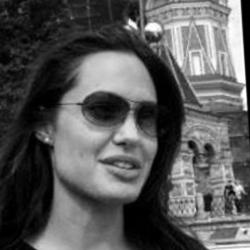
\includegraphics[width=\textwidth]{angelina/1}
        \end{subfigure}%
        ~ %add desired spacing between images, e. g. ~, \quad, \qquad etc.
        \begin{subfigure}[b]{0.2\textwidth}
                \centering
                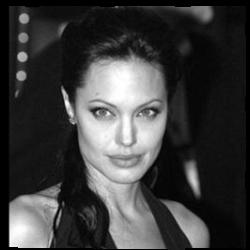
\includegraphics[width=\textwidth]{angelina/2}
        \end{subfigure}
        ~
        \begin{subfigure}[b]{0.2\textwidth}
                \centering
                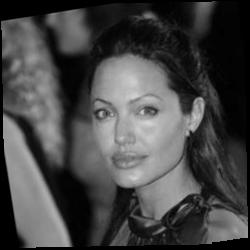
\includegraphics[width=\textwidth]{angelina/3}
        \end{subfigure}%
        ~ %add desired spacing between images, e. g. ~, \quad, \qquad etc.
        \begin{subfigure}[b]{0.2\textwidth}
                \centering
                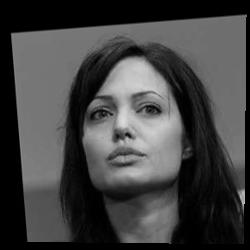
\includegraphics[width=\textwidth]{angelina/4}
        \end{subfigure}
%

        \begin{subfigure}[b]{0.2\textwidth}
                \centering
                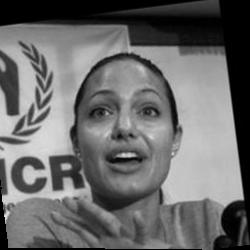
\includegraphics[width=\textwidth]{angelina/5}
        \end{subfigure}%
        ~ %add desired spacing between images, e. g. ~, \quad, \qquad etc.
        \begin{subfigure}[b]{0.2\textwidth}
                \centering
                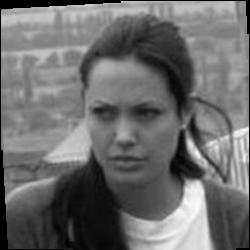
\includegraphics[width=\textwidth]{angelina/6}
        \end{subfigure}
        ~
        \begin{subfigure}[b]{0.2\textwidth}
                \centering
                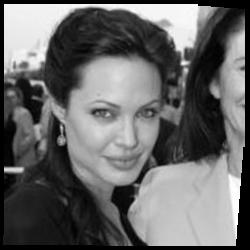
\includegraphics[width=\textwidth]{angelina/7}
        \end{subfigure}%
        ~ %add desired spacing between images, e. g. ~, \quad, \qquad etc.
        \begin{subfigure}[b]{0.2\textwidth}
                \centering
                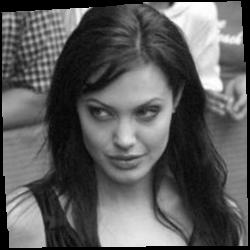
\includegraphics[width=\textwidth]{angelina/8}
        \end{subfigure}
%
        \begin{subfigure}[b]{0.2\textwidth}
                \centering
                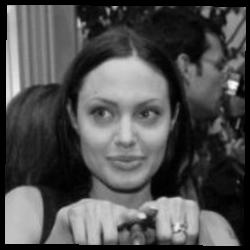
\includegraphics[width=\textwidth]{angelina/9}
        \end{subfigure}%
        ~ %add desired spacing between images, e. g. ~, \quad, \qquad etc.
        \begin{subfigure}[b]{0.2\textwidth}
                \centering
                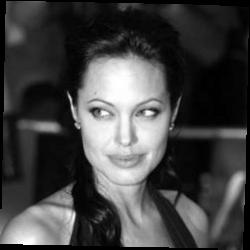
\includegraphics[width=\textwidth]{angelina/10}
        \end{subfigure}
        ~
        \begin{subfigure}[b]{0.2\textwidth}
                \centering
                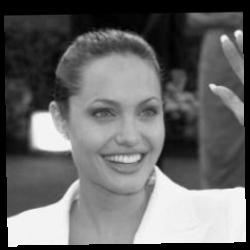
\includegraphics[width=\textwidth]{angelina/11}
        \end{subfigure}%
        ~ %add desired spacing between images, e. g. ~, \quad, \qquad etc.
        \begin{subfigure}[b]{0.2\textwidth}
                \centering
                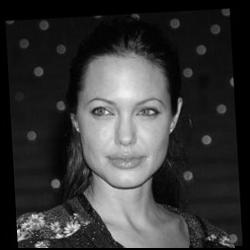
\includegraphics[width=\textwidth]{angelina/12}
        \end{subfigure}
%
        \begin{subfigure}[b]{0.2\textwidth}
                \centering
                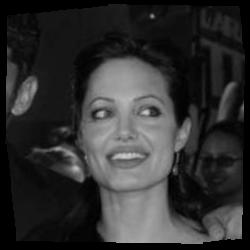
\includegraphics[width=\textwidth]{angelina/13}
        \end{subfigure}%
        ~ %add desired spacing between images, e. g. ~, \quad, \qquad etc.
        \begin{subfigure}[b]{0.2\textwidth}
                \centering
                
\includegraphics[width=\textwidth]{angelina/14}
        \end{subfigure}
        ~
        \begin{subfigure}[b]{0.2\textwidth}
                \centering
                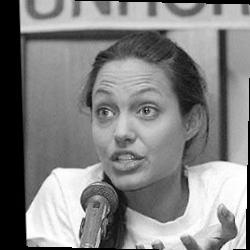
\includegraphics[width=\textwidth]{angelina/15}
        \end{subfigure}%
        ~ %add desired spacing between images, e. g. ~, \quad, \qquad etc.
        \begin{subfigure}[b]{0.2\textwidth}
                \centering
                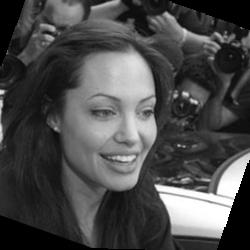
\includegraphics[width=\textwidth]{angelina/16}
        \end{subfigure}
        \caption{Exemplo de imagens do conjunto $\mathscr{G}$ para o sujeito Angelina Jolie}
        \label{fig:galeria}        
\end{figure}

A galeria de treino, $\mathscr{G}$, é constituída por 80\% das imagens de cada pessoa (16 imagens por pessoa), sendo as suas imagens utilizadas como amostras biométricas para o treino do sistema de reconhecimento facial. Um exemplo das imagens presentes na galeria de treino para o sujeito Angelina Jolie pode ser visto na figura \ref{fig:galeria}.

\begin{figure}
        \centering
        \begin{subfigure}[b]{0.2\textwidth}
                \centering
                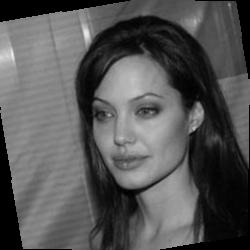
\includegraphics[width=\textwidth]{angelina/17}
        \end{subfigure}%
        ~ %add desired spacing between images, e. g. ~, \quad, \qquad etc.
        \begin{subfigure}[b]{0.2\textwidth}
                \centering
                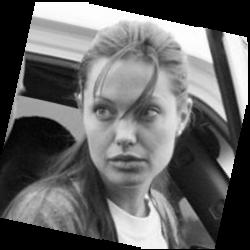
\includegraphics[width=\textwidth]{angelina/18}
        \end{subfigure}
        ~
        \begin{subfigure}[b]{0.2\textwidth}
                \centering
                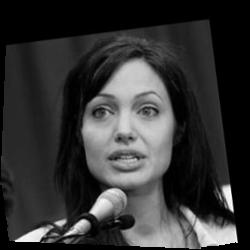
\includegraphics[width=\textwidth]{angelina/19}
        \end{subfigure}%
        ~ %add desired spacing between images, e. g. ~, \quad, \qquad etc.
        \begin{subfigure}[b]{0.2\textwidth}
                \centering
                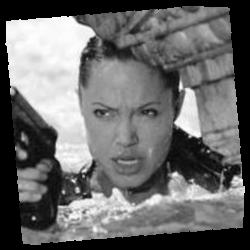
\includegraphics[width=\textwidth]{angelina/20}
        \end{subfigure}
        \caption{Exemplo de imagens do conjunto $\mathscr{P}$ para o sujeito Angelina Jolie}
        \label{fig:provas}   
\end{figure}

O conjunto $\mathscr{P}$ contem os restantes 20\% das imagens de cada pessoa (4 imagens por pessoa) e, tal como o seu nome indica, as suas imagens são utilizadas para a avaliação do sistema desenvolvido. Um exemplo das imagens presentes nas provas para o sujeito Angelina Jolie pode ser visto na figura \ref{fig:provas}.

As imagens incluídas na galeria de treino e nas provas, diferem também de forma aleatória entre os quatro conjuntos, tendo sido também selecionadas a partir da ferramenta \textit{GaleryCreator.exe}. A criação de 4 conjuntos com igual tamanho mas diferentes imagens de treino e teste tem em vista analisar o desempenho do sistema com diferentes galerias, de forma a determinar se existe uma variação significativa dos resultados obtidos em cada galeria.

\section{Pré-processamento} \label{sec:experiencias}
O módulo de reconhecimento facial, \textit{Face Recognizer}, disponibilizado pela plataforma \textit{OpenCV}, constituiu uma base sólida para o desenvolvimento do sistema de reconhecimento facial \textit{Visage}, contudo, de modo a tornar este sistema mais completo e versátil, revelou-se necessário adapta-lo e expandir as suas capacidades, nomeadamente através da aplicação de uma cadeia de pré-processamento às imagens existentes, tal como descrito na secção \ref{sec:facedetector} deste relatório. A evolução do sistema desenvolvido foi efetuada de forma gradual e iterativa, e culminou na construção de um conjunto de galerias de imagens, analisadas através de um grupo de experiências que permitem tirar conclusões acerca dos efeitos das diversas etapas de pré-processamento realizadas e da contribuição de cada uma delas para a melhoria do desempenho do sistema criado. 

Todas as galerias criadas possuem as imagens contidas nos conjuntos de teste definidos em \ref{sec:conjuntos}, diferenciando-se pelos diferentes passos de pré-processamento a que as imagens foram sujeitas. Na tabela \ref{tab:colecoes} encontram-se resumidas as galerias resultantes do conjunto de experiências efetuadas, as quais se encontram descritas pormenorizadamente de seguida.

\begin{center}
\begin{table}[ht]
	\caption{Galerias criadas após pré-processamento.}
	\begin{center}
    \begin{tabular}{l|cccc|c}
    \hline\hline
    Designação & Recortada   & Normalização           & Filtro Abstração & Máscara & Exemplo \\
	\hline
    Original   &   -         & -                      & -                &   -     & \ref{fig:original} \\
	~ & ~ & ~ & ~ & ~ & ~\\
    Cropped    & Sim         & -                      & -                &   -     & \ref{fig:cropped}  \\
    Masked     & Sim         & -                      & -                & Sim     & \ref{fig:masked}  \\
	~ & ~ & ~ & ~ & ~ & ~\\
    Normalized & Sim         & \textit{Constrast Streching}& -           & Sim     & \ref{fig:normalized}  \\
    Equalized  & Sim         & Equalização Histograma & -                & Sim     & \ref{fig:equalized}  \\
    CLAHE      & Sim         & \textit{CLAHE}         & -                & Sim     & \ref{fig:clahe}  \\
	~ & ~ & ~ & ~ & ~ & ~\\
    Bilateral  & Sim         & Equalização Histograma & Bilateral        & Sim     & \ref{fig:bilateral} \\
    Gaussian   & Sim         & Equalização Histograma & Gaussian         & Sim     & \ref{fig:gaussian}  \\
    AKF         & Sim        & Equalização Histograma & Kuwahara Anisotropico & Sim & \ref{fig:akf}     \\
    \hline\hline
    \end{tabular}
	\label{tab:colecoes}
	\end{center}
\end{table}
\end{center}

\subsection{Deteção e segmentação da face} \label{sec:pre-detecao}
Na revisão efetuada ao estado da arte do reconhecimento facial em imagens destacou-se a importância da resolução de um conjunto de sub-problemas específicos para um reconhecimento facial eficaz (ver \ref{sec:sub-problemas}), nomeadamente a deteção e segmentação das faces existentes numa imagem e  a remoção de elementos de fundo externos à imagem. Para a resolução deste problema, revelou-se necessário a avaliação de diferentes alternativas relativamente à forma como é efetuada a segmentação da face da restante imagem, assim como a determinação do impacto dessa segmentação no processo de reconhecimento.

Após uma análise das diferente alternativas existentes, e através de alguns teste intermédios realizados durante o período de desenvolvimento, foram então criadas as galerias de imagens Original, figura \ref{fig:original}; Cropped, figura \ref{fig:cropped}; e Masked, figura \ref{fig:masked}. A primeira, é constituída pelas imagens originais da biblioteca LFW-a e permite estabelecer uma base de comparação entre as imagens segmentadas e as imagens originais. A galeria cropped é composta por um conjunto de imagens onde as faces foram detetadas e segmentadas pelo detetor facial implementado e descrito no capítulo \ref{sec:facedetector}. A terceira e última galeria criada possui as mesmas imagens da galeria Cropped, sobre as quais foi posteriormente aplicada uma máscara elíptica de modo a aumentar a área de fundo removida das imagens recortadas.

\begin{figure}[t]
        \centering
        \begin{subfigure}[b]{0.2\textwidth}
                \centering
                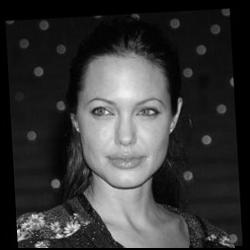
\includegraphics[width=\textwidth]{angelina/Angelina_Jolie_0006_original}
                \caption{Original}
                \label{fig:original-original} 
        \end{subfigure}%
%

        \begin{subfigure}[b]{0.2\textwidth}
                \centering
                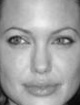
\includegraphics[width=\textwidth]{angelina/Angelina_Jolie_0006_cropped}
                \caption{Cropped}
                \label{fig:cropped} 
        \end{subfigure}
        ~ ~
        \begin{subfigure}[b]{0.2\textwidth}
                \centering
                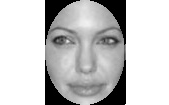
\includegraphics[width=\textwidth]{angelina/Angelina_Jolie_0006_masked}
                \caption{Masked}
                \label{fig:masked}
        \end{subfigure}%
%

        \begin{subfigure}[b]{0.2\textwidth}
                \centering
                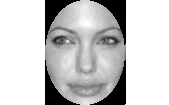
\includegraphics[width=\textwidth]{angelina/Angelina_Jolie_0006_normalized}
                \caption{Normalized}
                \label{fig:normalized} 
        \end{subfigure}
        ~ ~
        \begin{subfigure}[b]{0.2\textwidth}
                \centering
                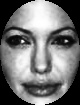
\includegraphics[width=\textwidth]{angelina/Angelina_Jolie_0006_equalized}
                \caption{Equalized}
                \label{fig:equalized}
        \end{subfigure}
        ~ ~
        \begin{subfigure}[b]{0.2\textwidth}
                \centering
                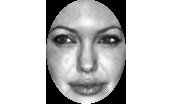
\includegraphics[width=\textwidth]{angelina/Angelina_Jolie_0006_CLAHE}
                \caption{CLAHE}
                \label{fig:clahe}
        \end{subfigure}
        %
        
        \begin{subfigure}[b]{0.2\textwidth}
                \centering
                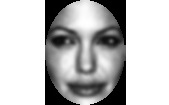
\includegraphics[width=\textwidth]{angelina/Angelina_Jolie_0006_gaussian}
                \caption{Gaussian}
                \label{fig:gaussian} 
        \end{subfigure}
        ~ ~
        \begin{subfigure}[b]{0.2\textwidth}
                \centering
                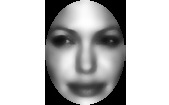
\includegraphics[width=\textwidth]{angelina/Angelina_Jolie_0006_bilateral}
                \caption{Bilateral}
                \label{fig:bilateral}
        \end{subfigure}
        ~ ~
        \begin{subfigure}[b]{0.2\textwidth}
                \centering
                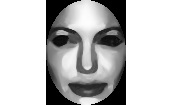
\includegraphics[width=\textwidth]{angelina/Angelina_Jolie_0006_akf}
                \caption{AKF}
                \label{fig:akf}
        \end{subfigure}
        \caption{Variação da mesma imagem nos vários conjuntos pré-processados analisados.}
        \label{fig:galeriaspreprocessadas}   
\end{figure}

\subsection{Normalização do Contraste} \label{sec:pre-normalizacao}
A normalização das imagens em termos de contraste é passo comum e essencial à maioria dos sistemas de reconhecimento facial automático modernos, tal como destacado no capítulo \ref{chap:reco} desta dissertação. Assim sendo, no decorrer do desenvolvimento do sistema de reconhecimento facial Visage, revelou-se também importante analisar o qual o impacto da normalização do contraste nas imagens utilizadas, assim como qual a melhor forma de efetuar a sua normalização. Foram então estudadas três formas distintas de efetuar a normalização do contraste, \textit{Contrast Streching}, Equalização Histograma e \textit{CLAHE}, descritas em \ref{sec:normalizacao}.

Da aplicação da técnica de contrast streching às imagens presentes nos conjuntos de teste descritos anteriormente resultou a criação da galeria Normalized. As imagens normalizadas através da equalização simples do histograma encontram-se representadas na galeria Equalized e as normalizadas pela técnica \textit{CLAHE} encontram-se representadas na galeria com o mesmo nome. Para além de normalizadas, as imagens foram também recortadas e após o seu processamento fou aplicada uma máscara elíptica sobre as mesmas. As figuras \ref{fig:normalized}, \ref{fig:equalized} e \ref{fig:clahe} representam exemplos da aplicação das três técnicas avaliadas sobre a mesma imagem.

\subsection{Abstração Imagens} \label{sec:pre-abstração}
O último conjunto de galerias criadas visa analisar a hipótese levantada no âmbito desta dissertação, acerca do impacto do uso de filtros de abstração no reconhecimento facial em imagens. 
A utilização de filtros de abstração constitui uma forma moderna de simplificação do conteúdo visual, permitindo remover informação redundante e aumentar o destaque da mensagem visual a transmitir. Estudos efetuados demonstraram que a aplicação destes filtros na recuperação de informação multimédia, nomeadamente no âmbito da da ilustração automática de texto têm a potencialidade de melhorar a informação retornada, assim como reduzir significativamente as necessidades de processamento e armazenamento das imagens \cite{Coelho2012}. O uso de filtros de abstração no âmbito do sistema Visage, tem em vista analisar qual o impacto do uso destes filtros no reconhecimento facial em imagens, quer ao nível do desempenho do sistema, quer ao nível das suas necessidades de armazenamento e processamento das imagens.

Para além de abstraídas as imagens foram também sujeitas às tarefas de pré-processamento que apresentaram melhores resultados nos conjuntos anteriormente criados, nomeadamente a deteção e segmentação da face, a normalização do seu histograma e ainda a aplicação de uma máscara após a aplicação do filtro de abstração.

A abstração das imagens foi efetuada com recurso aos filtros gaussiano, bilateral e kuwahara anisotrópico, descritos em \ref{sec:filtros}, resultando na criação das galerias Gaussian, Bilateral e AKF, respectivamente.

\section{Avaliação \textit{Closed-Set Identification}} \label{sec:avaliacao1}
Tal como introduzido na secção \ref{sec:problema}, o paradigma de \textit{closed-set identification}, constitui um sub-problema de identificação em que uma prova é apresentada ao sistema e pretende-se que este devolva a identidade da pessoa presente na imagem. Neste caso particular do problema de identificação, todas as provas apresentadas possuem uma correspondência na galeria, em oposição ao caso geral de identificação, no qual pode ou não haver uma correspondência.

A avaliação \textit{closed-set} é uma medida padrão de avaliação do desempenho em sistemas de reconhecimento facial automático, tendo sido utilizada em diversas avaliações efetuadas, nomeadamente nas avaliações FERET e FRVT apresentadas na revisão do estado da arte desta dissertação (ver \ref{chap:reco}). A utilização de um conjunto fechado de imagens permite uma análise detalhada do desempenho de um algoritmo permitindo responder à pergunta "a identificação correta encontra-se nos primeiros $n$ resultados? " em vez de apenas " o primeiro resultado é o correto?".

\subsection{Metodologia Avaliação}
Para cada conjunto de teste descrito em \ref{sec:conjuntos}, seja $\mathscr{G}$ a sua galeria de treino, em que $\mathscr{G} = \{g_1, ..., g_N\}$ e seja $\mathscr{P}$ o conjunto das suas provas, em que $\mathscr{P} = \{p_1, ..., p_N\}$. Quando uma prova $p_j$ é apresentada ao sistema, essa prova é então comparada a cada amostra biométrica $g_i$ da galeria, resultando dessa comparação o respetivo índice de similaridade (\textit{similarity score}), $s_{ij}$. Este índice é designado de $match$ $score$, caso $g_i$ e $p_j$ sejam amostras da mesma pessoa, caso não o sejam é designado de $nonmatch$ $score$. Quanto menor o índice de similaridade, maior é a probabilidade das imagens comparadas pertencerem à mesma pessoa, sendo que o melhor valor possível para o índice de similaridade de um $match$ $score$ é zero.

Na identificação de $p_j \in \mathscr{P}$, em primeiro lugar são calculados os índices de similaridade para todas as amostras na galeria $\mathscr{G}$, sendo posteriormente ordenados os seus resultados. O ranking de $p_j$, $r_{p_j}$, é igual a $n$, se o seu $match$ $score$ corresponde ao enésimo menor índice de similaridade. A taxa de identificação para o ranking $n$, $T_{I}(n)$, corresponde à fração de provas com ranking $n$ ou menor do que $n$, ou seja:
\begin{equation}
T_{I}(n) = \frac{|C(n)|}{|\mathscr{P}|} \times 100
\end{equation}
Em que $|C(n)|$ é número de provas com ranking $n$, ou menor do que $n$, e $|\mathscr{P}|$ o número de provas existentes em $\mathscr{P}$.

A $T_{I}(n)$ é calculada para todos os rankings entre 1 e 30. Dentro desse intervalo, os primeiros níveis de ranking apresentam uma maior variação na percentagem de pessoas identificadas, revelando-se assim mais significativos para a análise do desempenho do sistema.

A avaliação é efetuada através da análise do desempenho dos três algoritmos disponíveis em cada uma das galerias de imagens pré-processadas, encontrando-se os resultados obtidos agrupados num conjunto de três experiências, cada uma dedicada a analisar a variação do comportamento do sistema dado um problema específico, utilizando para isso diferentes grupos de galerias de imagens pré-processadas. A divisão entre imagens de treino e teste de cada galeria é efetuada segundo os quatro conjuntos de testes criados, sendo cada galeria avaliada em cada um dos quatro conjuntos de teste existentes e posteriormente calculada a média dos resultados obtidos.

A média dos resultados obtidos encontra-se representada em um gráfico do tipo \textit{Cumulative match score} (CMS). Um gráfico do tipo CMS representa $T_{I}(n)$ como uma função de ranking $n$. No eixo horizontal encontra-se representado o ranking e no eixo vertical encontra-se representada a respetiva taxa de identificação, um exemplo de um gráfico CMS pode ser visto em \ref{fig:exp1_comaparacao}.

\subsection{Resultados Experiência 1: Impacto da segmentação das faces}

\begin{figure}[p]
        \centering
        \begin{subfigure}[b]{0.58\textwidth}
                \centering
                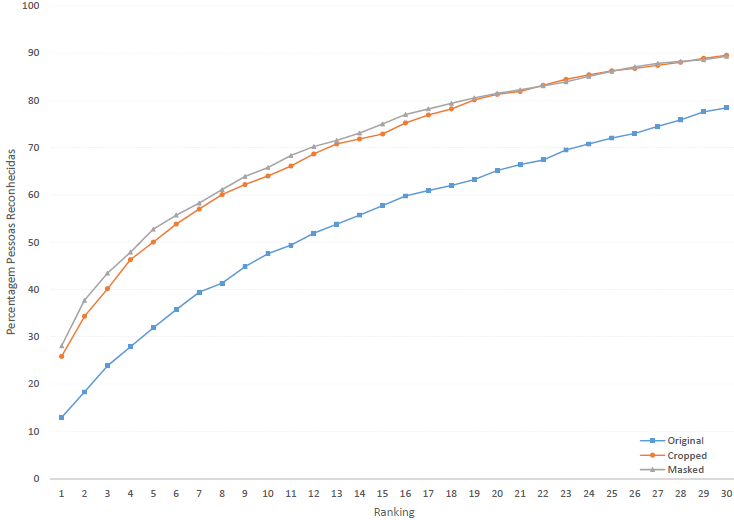
\includegraphics[width=\textwidth]{resultados/original_cropped_masked_eigen}
                \caption{Eigenfaces}
                \label{fig:original_cropped_masked_eigen}
        \end{subfigure}%

        \begin{subfigure}[b]{0.58\textwidth}
                \centering
                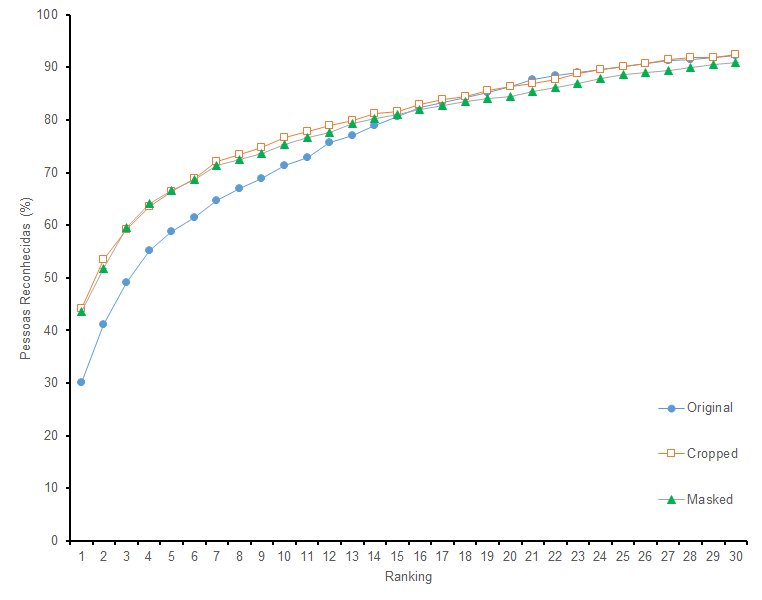
\includegraphics[width=\textwidth]{resultados/original_cropped_masked_fisher}
                \caption{Fisherfaces}
                \label{fig:original_cropped_masked_fisher}
        \end{subfigure}

        \begin{subfigure}[b]{0.58\textwidth}
                \centering
                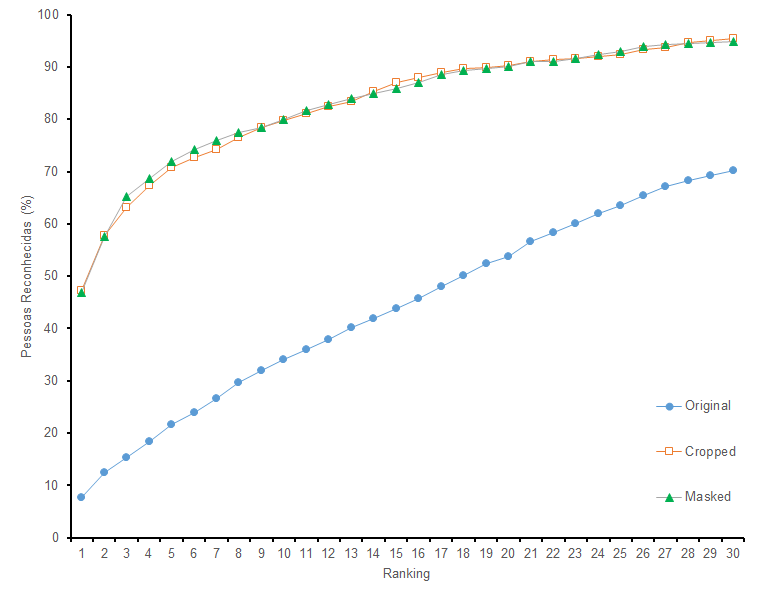
\includegraphics[width=\textwidth]{resultados/original_cropped_masked_lbph}
                \caption{LBPH}
                \label{fig:original_cropped_masked_lbph}
        \end{subfigure}
        \caption{Desempenho algoritmos Eigenfaces, Fisherfaces e LBPH para os conjuntos Original, Cropped e Masked}
        \label{fig:original_cropped_masked}
\end{figure}

Esta experiência visa analisar o impacto da segmentação das faces presentes na imagem do fundo existente nas mesmas. Os resultados obtidos podem ser visualizados na figura \ref{fig:original_cropped_masked}, onde se encontram ilustrada a performance dos algoritmos, \textit{Eigenfaces}, \textit{Fisherfaces} e \textit{LBPH}, nos três conjuntos criados especialmente para esta experiência, os quais se encontram descritos mais pormenorizadamente em \ref{sec:pre-detecao}.

Após a analise dos resultados obtidos na experiência 1, nomeadamente através da comparação das taxa de identificação de ranking 1 dos conjuntos Cropped e Masked com o conjunto Original, verifica-se que a segmentação das faces presentes nas imagens originais produz uma melhoria efetiva dos resultados obtidos, traduzindo-se num aumento de cerca de 12\%, 14\% e 40\% para os algoritmos \textit{Eigenfaces}, \textit{Fisherfaces} e \textit{LBPH}, respetivamente.

Uma análise mais aprofundada desses resultados, demonstra ainda que, no caso dos algoritmos \textit{Eigenfaces} e \textit{LBPH}, a diferença na taxa de identificação entre as imagens originais (conjunto Original) e as imagens segmentadas (conjuntos Cropped e Masked) é significativa e relativamente constante nos vários níveis para os quais a taxa de deteção se encontra reportada. Por outro lado, no caso do algoritmo \textit{Fisherfaces}, apesar da diferença significativa no número de imagens corretamente identificadas nos primeiros níveis, a partir do ranking 15, todos os conjuntos de imagens obtém uma taxa de identificação similar, e com uma progressão semelhante. Esta aproximação no número de caras corretamente identificadas nos rankings mais elevados pode ser explicada pela existência de informação no fundo das imagens, a qual poderá ser utilizada pelo próprio algoritmo para a identificação das mesmas, ao invés da utilização da face contida na imagem, reforçando assim a importância da extração do fundo contido nas imagens originais.

Por outro lado, note-se ainda que, apesar do impacto positivo da segmentação das imagens nos três algoritmos testados, o impacto desta segmentação varia significativamente conforme o algoritmo utilizado, sendo que o \textit{Fisherfaces} é o que revela resultados mais constantes independentemente da manipulação efetuada nas imagens e o algoritmo \textit{LBPH} o que regista uma maior melhoria desses mesmos resultados.

Ao nível da diferença entre as imagens apenas segmentadas (conjunto Cropped) e as imagens com máscara (conjunto Masked), é possível verificar que ambas possuem resultados semelhantes, sendo que a maior diferença foi detetada no algoritmo \textit{Eigenfaces}, onde as imagens com máscara demonstraram um desempenho ligeiramente superior, como é possível verificar pelas $T_{I}(2)$ de 43,4\% e 40,1\% para as imagens com máscara e apenas recortadas, respetivamente. Apesar da diferença registada não ser muito significativa, a existência de uma máscara garante uma extração de uma maior quantidade de fundo das imagens, permitindo assim uma maior confiança dos resultados obtidos, no sentido em que se reduz o perigo de identificação pelas características do fundo da imagem e não das caraterísticas faciais presentes na mesma. 

\begin{figure}[ht]
  \begin{center}
    \leavevmode
    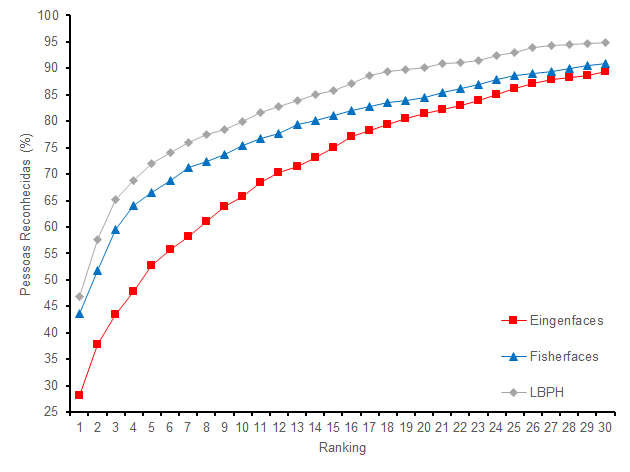
\includegraphics[width=0.6\textwidth]{resultados/exp1_comparacao}
    \caption{Comparação do desempenho dos três algoritmos implementados para o conjunto Masked}
    \label{fig:exp1_comaparacao}
  \end{center}
\end{figure}

Finalmente, através da análise do gráfico \ref{fig:exp1_comaparacao}, é possível concluir que ao nível dos algoritmos utilizados o algoritmo \textit{LBPH} obtém resultados globalmente melhores, ao passo que o algoritmo \textit{Eingefaces} obtém os piores resultados. Esta diferença verifica-se quer nos rankings inferiores, quer nos superiores, sendo menor quanto maior é o ranking utilizado, como é possível verificar pelas taxas de identificação de ranking 1 de 46,8\% e 28,1\%, no conjunto Masked, para os algoritmos \textit{LBPH} e \textit{Eigenfaces}, respetivamente, e pelas taxas de identificação de ranking 30 de 94,9\% e 89,3\%, para os mesmos algoritmos no mesmo conjunto. A análise comparativa do desempenho dos três algortimos encontra-se reportada no gráfico \ref{fig:exp1_comaparacao} para a galeria masked, uma vez esta foi a galeria que revelou melhores resultados das três analisadas.

\subsection{Resultados Experiência 2: Impacto da Normalização do Contraste} \label{sec:avaliacao2-exp2}
\begin{figure}[p]
        \centering
        \begin{subfigure}[b]{0.58\textwidth}
                \centering
                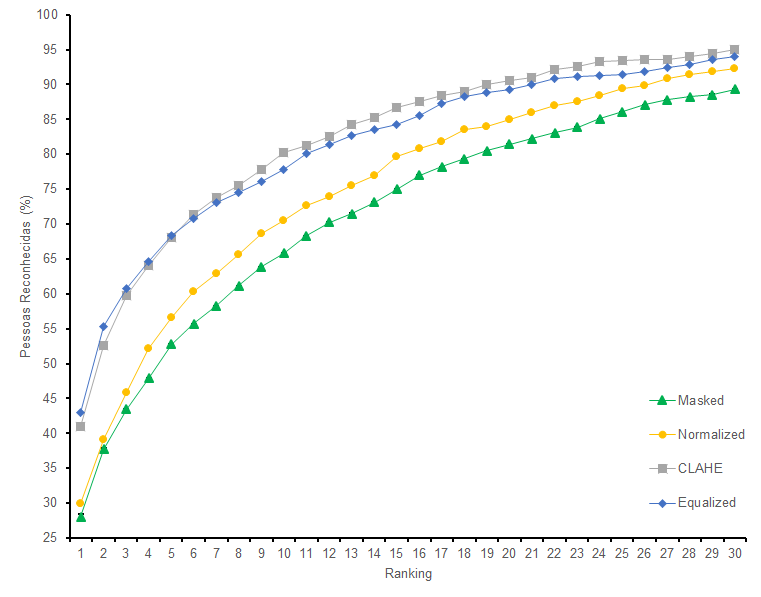
\includegraphics[width=\textwidth]{resultados/Exp_2_eigen}
                \caption{Eigenfaces}
                \label{fig:masked_normalized_equalized_clahe_eigen}
        \end{subfigure}%

        \begin{subfigure}[b]{0.58\textwidth}
                \centering
                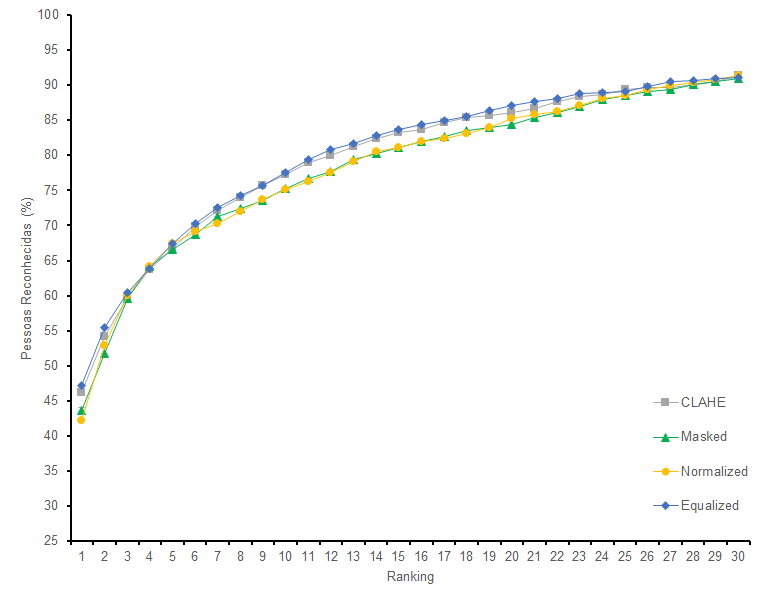
\includegraphics[width=\textwidth]{resultados/Exp_2_fisher}
                \caption{Fisherfaces}
                \label{fig:masked_normalized_equalized_clahe_fisher}
        \end{subfigure}

        \begin{subfigure}[b]{0.58\textwidth}
                \centering
                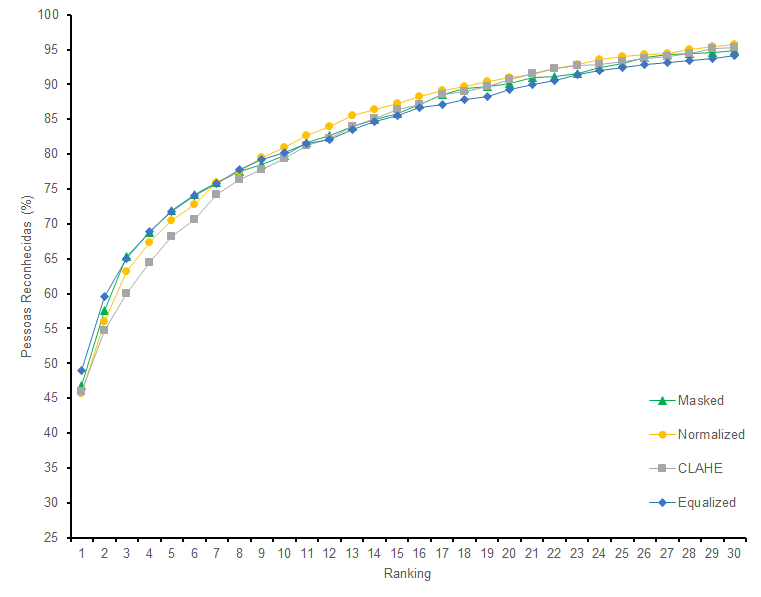
\includegraphics[width=\textwidth]{resultados/Exp_2_lbph}
                \caption{LBPH}
                \label{fig:masked_normalized_equalized_clahe_lbph}
        \end{subfigure}
        \caption{Desempenho algoritmos Eigenfaces, Fisherfaces e LBPH para os conjuntos Normalized, Equalized e CLAHE}
        \label{fig:exp2}
\end{figure}

A aquisição de imagens em condições não controladas pode resultar na obtenção de fotografias com um contraste reduzido e níveis de iluminação muito distintos. De forma a ultrapassar este problema, a normalização do contraste de uma imagem é uma tarefa comum nos sistemas de reconhecimento faciais modernos. Nesta experiência pretendemos analisar qual o impacto da normalização do contraste de uma imagem nos diferentes algoritmos implementados, assim como determinar qual a melhor estratégia de normalização, de entre três técnicas distintas implementadas, através da analise do desempenho do sistema em três galerias previamente normalizadas com cada uma dessas técnicas (ver \ref{sec:pre-normalizacao}).

Na figura \ref{fig:exp2} é possível visualizar os resultados para obtidos para o desempenho do sistema nas galerias Normalized, Equalized e CLAHE, correspondentes às técnicas de normalização \textit{contrast stretching}, equalização histograma e CLAHE, respectivamente, as quais encontram-se descritas na secção \ref{sec:normalizacao} deste relatório. Nos gráficos da figura \ref{fig:exp2} encontra-se ainda representados os resultados obtidos para o conjunto Masked, utilizado na experiência 1, o qual serve de referência para a comparação entre os conjuntos não normalizados e os conjuntos normalizados.

Como é possível concluir pela observação da figura \ref{fig:exp2}, a normalização das imagens apresenta resultados globalmente melhores do que os obtidos para conjuntos não normalizados. O impacto obtido varia, no entanto, consideravelmente conforme o algoritmo utilizado, sendo que o maior impacto é registado para o algoritmo Eigenfaces, onde existe uma melhoria na ordem dos 15.0\% na percentagem de pessoas reconhecidas no primeiro nível do ranking, quando comparadas as galerias Masked e Equalized. Os algoritmos \textit{Fisherfaces} e \textit{LBPH} mostram uma diferença máxima de apenas 3.8\% e 2.2\% entre os conjuntos Masked e Equalized, pelo que é possível concluir que estes algoritmos possuem uma maior resistência aos efeitos da iluminação no desempenho quando comparados com o algoritmo \textit{Eigenfaces} \footnote{A pouca variação obtida neste dois últimos algoritmos vai de acordo com o defendido por investigações anteriores realizadas por \cite{ahonen2004face}.}.

Ao nível das três técnicas utilizadas é possível concluir que as duas variantes de equalização do histograma possuem os resultados mais satisfatórios. A equalização simples do histograma, conjunto Equalized, tem tendência a demonstrar resultados melhores para os primeiros níveis de ranking, sendo posteriormente igualada ou até ultrapassada pela técnica CLAHE nos níveis mais superiores. Uma vez que os primeiros níveis de ranking incluem a informação mais significativa para a maioria dos utilizadores de sistemas de reconhecimento facial automático, consideramos que o desempenho da equalização do histograma das imagens possuí resultados mais relevantes para a utilização no sistema de reconhecimento facial Visage do que a técnica \textit{CLAHE}.

\begin{figure}[ht]
  \begin{center}
    \leavevmode
    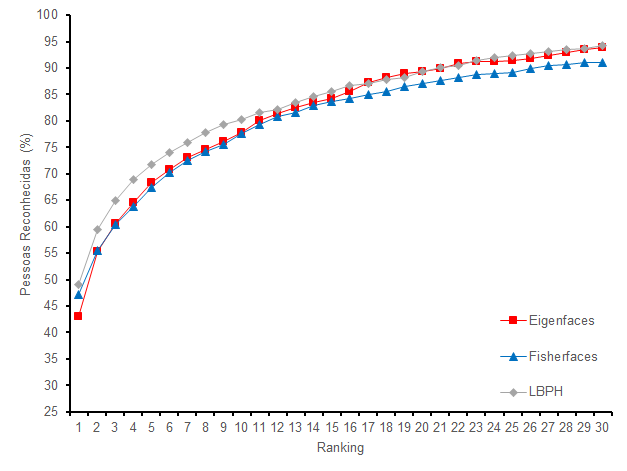
\includegraphics[width=0.6\textwidth]{resultados/exp2_comparacao}
    \caption{Comparação do desempenho dos três algoritmos implementados para o conjunto Equalized}
    \label{fig:exp2_comaparacao}
  \end{center}
\end{figure}

Finalmente, a análise comparativa dos resultados obtidos para os três algoritmos implementados, ilustrada pelo gráfico \ref{fig:exp2_comaparacao}, permite concluir que após a normalização do histograma das imagens o desempenho dos algoritmos apresenta uma diferença muito menor do que a registada anteriormente e ilustrada pelo gráfico \ref{fig:exp1_comaparacao}. Nesta experiência o algoritmo LBPH continua a ser o algoritmo com melhor desempenho, registando no entanto uma diferença de apenas 1.8\% e 6.0\% para os algoritmos \textit{Fisherfaces} e \textit{Eigenfaces}, respetivamente, na taxa de identificação de ranking 1 no conjunto Equalized. De notar ainda que, a partir do ranking de nível 2, o algoritmo  \textit{Eigenfaces} possui uma taxa de identificação idêntica ao valores obtidos pela algoritmo \textit{Fisherfaces}, ultrapassando o desempenho do segundo, a partir do ranking 11. Esta grange evolução no desempenho, notada para o algoritmo \textit{Eigenfaces}, em contraste com a ligeira melhoria obtida pelos restantes denota a complexidade associada ao problema de reconhecimento facial automático, nomeadamente no que diz respeito à forma como diferentes fatores afetam de forma diferenciada diferentes algoritmos e diferentes conjuntos de dados.

\subsection{Resultados Experiência 3: Abstração de Imagens}
A terceira e última experiência realizada visa analisar qual o impacto da utilização de filtros de abstração no processo de reconhecimento facial em imagens. A análise foi efetuada com recurso a três filtros de abstração diferentes, descritos em \ref{sec:filtros}, os quais correspondem a diferentes técnicas e níveis de abstração, sendo o filtro gaussiano o filtro com um menor impacto na imagem original e o filtro kuwahara anisotróprico aquele que produz um maior grau de abstração. 

Os resultados da análise de desempenho efetuada nesta terceira experiência encontram-se representados na figura \ref{fig:exp3} em quatro galerias distintas. A primeira corresponde à galeria Equalized, utilizada na experiência 2, e que serve como referência de comparação entre as imagens abstraídas e as imagens normalizadas, uma vez que esta foi a galeria onde se registou o melhor desempenho na experiência 2. Da aplicação dos filtros de abstração nas imagens existentes na galeria Equalized, resultou a criação de três galerias distintas Gaussian, na qual foi utilizado o filtro gaussiano para  a abstração das imagens, Bilateral, na qual foi utilizado o filtro homónimo para a abstração das imagens e ainda a galeria AKF cujas imagens foram abstraídas com recurso ao filtro kuwahara anisotrópico. Uma descrição mais pormenorizada destas galerias pode ser encontrada em \ref{sec:pre-abstração}.

\begin{figure}[p]
        \centering
        \begin{subfigure}[b]{0.58\textwidth}
                \centering
                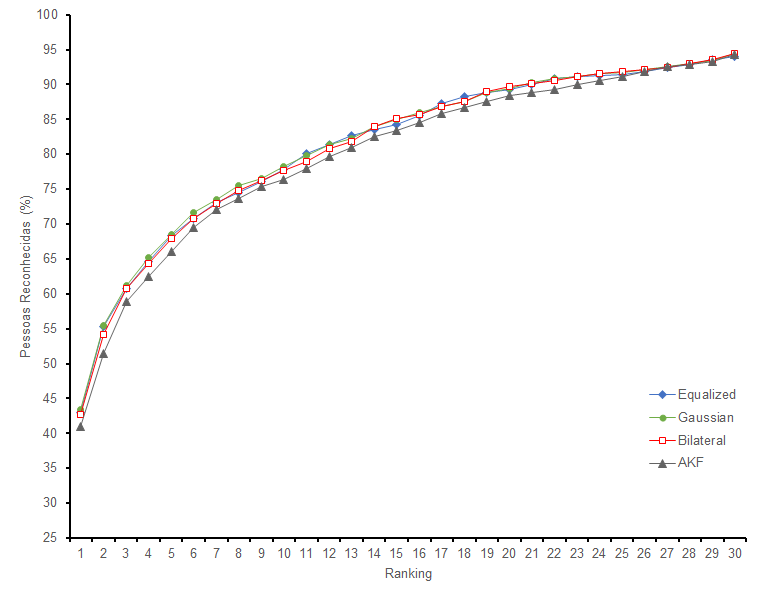
\includegraphics[width=\textwidth]{resultados/Exp_3_eigen}
                \caption{Eigenfaces}
                \label{fig:exp3_eigen}
        \end{subfigure}%

        \begin{subfigure}[b]{0.58\textwidth}
                \centering
                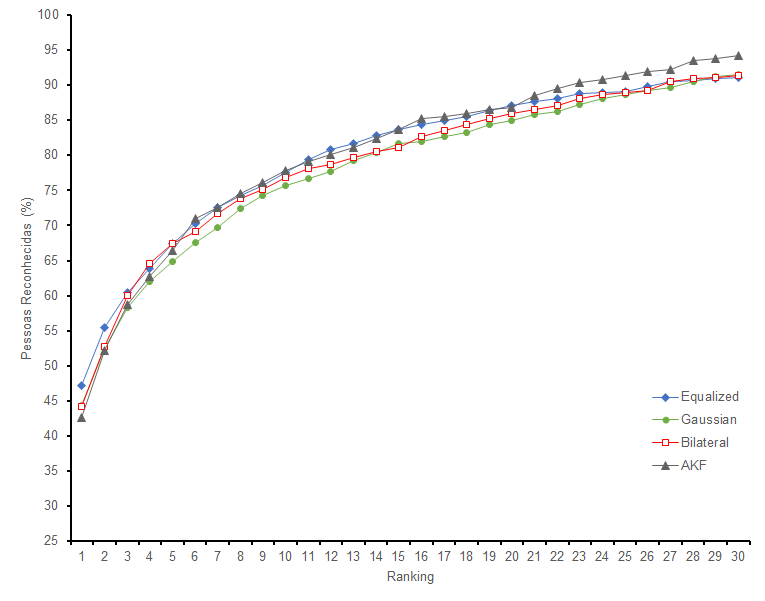
\includegraphics[width=\textwidth]{resultados/Exp_3_fisher}
                \caption{Fisherfaces}
                \label{fig:exp3_fisher}
        \end{subfigure}

        \begin{subfigure}[b]{0.58\textwidth}
                \centering
                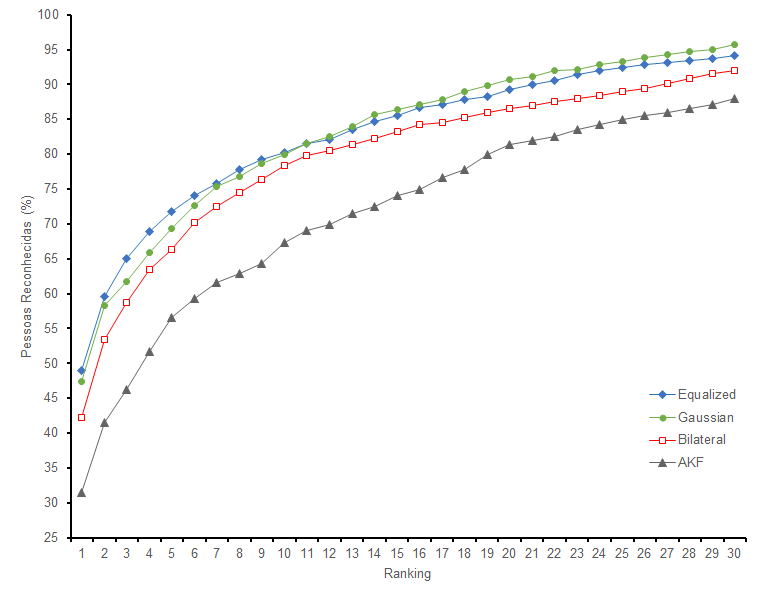
\includegraphics[width=\textwidth]{resultados/Exp_3_lbph}
                \caption{LBPH}
                \label{fig:exp3_lbph}
        \end{subfigure}
        \caption{Desempenho algoritmos Eigenfaces, Fisherfaces e LBPH para os conjuntos Gaussian, Bilateral e AKF}
        \label{fig:exp3}
\end{figure}

A análise da figura \ref{fig:exp3} permite concluir que, de uma forma global, não se verifica um melhoria significativa nos resultados obtidos com o recurso à abstração de imagens no desempenho do sistema de reconhecimento facial criado. 

O impacto do uso da abstração de imagens varia, no entanto, conforme o algoritmo de reconhecimento utilizado. O algoritmo \textit{Eigenfaces} é o que regista uma menor variação nos resultados obtidos quando comparadas taxas de identificação registadas nas galerias abstraídas com as registadas para a coleção Equalized. A este nível as galerias Gaussian e Bilateral registam um desempenho equivalente ao conjunto de imagens Equalized, enquanto que a galeria AKF regista um desempenho ligeiramente inferior, como é possível verificar pelas taxas de identificação nível 1 de 43.0\%, 43.4\%, 42.7\% para as galerias Equalized, Gaussian e Bilateral e 41.0\% para a galeria AKF.

Para o algoritmo \textit{Fisherfaces} a galeria abstraída com recurso ao filtro gaussiano é a que regista um pior desempenho, obtendo uma taxa de identificação inferior, ou equivalente às restantes galerias em todos os níveis para os quais a taxa de identificação se encontra reportada. As galerias Bilateral e AKF, apresentam um desempenho equivalente ao da galeria Equalized, sendo que no caso do conjunto Bilateral o desempenho é regra geral ligeiramente inferior ao das outras duas galerias, ao passo que o o conjunto AKF regista uma melhoria considerável no número de pessoas identificadas a partir do ranking 20 até ao final, como é possível verificar pelas taxas de identificação de ranking 30 de cerca de 91\% para os conjuntos Equalized, Gaussian e Bilateral e de 94.2\% para o conjunto AKF.

Finalmente, o algoritmo \textit{LBPH} é o que regista um maior impacto na utilização da abstração de imagens no processo de reconhecimento, sendo que nos casos dos conjuntos Bilateral e AKF o desempenho do reconhecimento piora significativamente, registando valores 6.8\% inferiores para a taxa de identificação nível 1 no conjunto Bilateral e 17.6\% inferiores para o mesmo ranking na comparação entre o conjunto AKF e Equalized. No caso do conjunto Gaussian, o desempenho é equivalente ou ligeiramente inferior do que o registado para o conjunto Equalized até ao ranking 6, passando a ser ligeiramente superior a partir deste nível até ao final onde é registada um diferença de 1.5 pontos na percentagem de pessoas identificadas.


\begin{figure}[ht]
  \begin{center}
    \leavevmode
    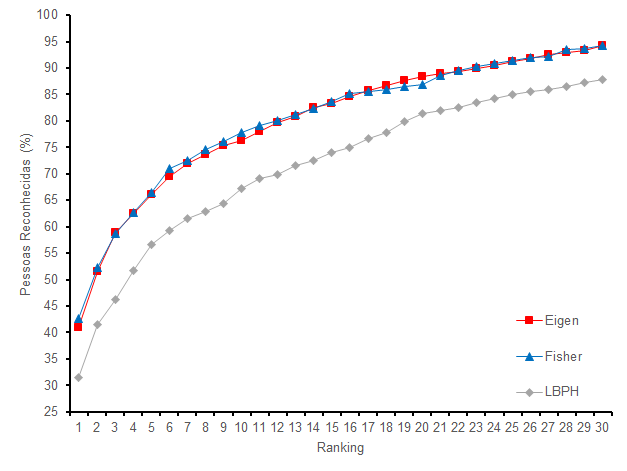
\includegraphics[width=0.6\textwidth]{resultados/exp3_comparacao}
    \caption{Comparação do desempenho dos três algoritmos implementados para o conjunto AKF}
    \label{fig:exp3_comaparacao}
  \end{center}
\end{figure}

\section{Avaliação \textit{Image Retrieval}} \label{sec:avaliacao2}
A metodologia de avaliação proposta na secção \ref{sec:avaliacao1} desta dissertação permite-nos efetuar uma avaliação qualitativa do desempenho do sistema de reconhecimento facial criado, assim como dos diferentes algoritmos implementados, através de uma medida padrão para a avaliação de sistemas de reconhecimento facial automáticos. Nesta segunda avaliação propomos a avaliação do desempenho do sistema de um ponto de vista centrado num possível caso de uso do mesmo: \textit{Image Retrieval}.

A área de recuperação de informação multimédia regista atualmente uma importância crescente, resultado do elevado número de conteúdos produzidos, assim como do elevado número de dispositivos de partilha disponíveis, tal como destacado na revisão do estado da arte desta dissertação. Desta forma, a recuperação de informação multimédia e em particular a área de \textit{Image Retrieval} representa uma das áreas com maior potencial para a utilização do sistema de reconhecimento facial criado.

Para uma dada imagem contendo uma face, o sistema Visage é capaz de detetar a face presente na imagem e apresentar uma lista ordenada de possíveis entidades que se encontram representadas nessa imagem, de acordo com um modelo anteriormente treinado. Com base neste sistema é possível desenvolver aplicações de \textit{image retrieval} capazes de encontrar fotos de uma personalidade específica ou apresentar, para uma foto de rosto fornecida pelo utilizador, a celebridade ou figura pública mais parecida.

\subsection{Metodologia Avaliação}
Em recuperação de informação multimédia designa-se de \textit{precisão} a fração de documentos relevantes do total de documentos retornados por uma pesquisa. Ao analisar a precisão podem ser analisados todos os documentos relevantes ou apenas os $n$ documentos mais relevantes, designado-se nessa situação de \textit{precisão a n}.

No sistema de reconhecimento facial criado, para uma dada imagem é apresentada uma lista de possíveis entidades que se encontram representadas nessa imagem, em que o primeiro resultado representa a entidade com maior probabilidade de estar presente na imagem e em que cada entidade aparece uma única vez na lista de resultados possíveis. Caso se pretenda efetuar a identificação de uma personalidade existe apenas um resultado verdadeiramente relevante na lista de resultados obtida, pelo que a medida de \textit{precisão a n} utilizada em recuperação de informação multimédia não é válida para a avaliação efetuada nesta secção.

Para avaliação do desempenho do sistema do ponto de vista de \textit{image retrieval} foi então criada a medida \textit{precisão na galeria} (PG). A \textit{precisão na galeria} resulta da adaptação da precisão de recuperação de informação multimédia ao caso particular do sistema de reconhecimento facial automático desenvolvido. Considerando a definição de ranking de uma prova apresentada em \ref{sec:avaliacao1}, a \textit{precisão na galeria} de $p_j$, $PG_{p_j}$, corresponde a:

\begin{equation}
PG_{p_j} = \frac{1}{r_{p_j}} \times 100
\end{equation}

Em que $\mathscr{P}$ é o conjunto de provas da galeria, $p_j \in \mathscr{P}$ e $r_{p_j}$ corresponde ao ranking da prova $p_j$.

A \textit{precisão na galeria} de uma prova progride então de 100\% para ranking 1, 50\% para ranking 2, 33\% ranking 3 e assim sucessivamente. As provas com um menor ranking têm então uma maior precisão, assim como uma maior distância entre si em termos de precisão (50 unidades entre 1 e 2, 22 unidades entre 2 e 3, e assim sucessivamente). Ora, no caso de \textit{image retrieval} é importante que o resultado mais relevante, a identificação correta de uma pessoa, surja com o menor ranking possível, pelo que a distância nas \textit{precisões na galeria} obtidas nos primeiros resultados deve ser maior do que a obtida para os resultados que surgem posteriormente na lista de entidades possíveis, tal como verificado na métrica adotada. Desta forma, é possível analisar a desempenho do sistema com ênfase nos resultados de topo para uma determinada prova, beneficiando os valores de \textit{precisão na galeria} quando o nome correto aparece cedo na lista de resultado possíveis, ao mesmo tempo que se diferencia significativamente os resultados de topo.

Dada a \textit{precisão na galeria} a \textit{média da precisão na galeria} (MPG) de um algoritmo é calculada através da média da \textit{precisão na galeria} obtida para cada prova, ou seja:
\begin{equation}
MPG_{algoritmo} = \frac{ \sum\limits_{i=0}^{n} PG_{p_i} }{n}
\end{equation}

Em que $n$ corresponde ao número de provas existentes em $\mathscr{P}$.

Através da \textit{média da precisão na galeria} é possível analisar o desempenho de um algoritmo de uma forma global, ao contrário da avaliação efetuada em  \ref{sec:avaliacao1}, onde o desempenho de um algoritmo é analisado em função da progressão da sua taxa de identificação em vários rankings.

\subsection{Resultados}

\begin{center}
\begin{table}
    \begin{center}
    \caption{Resultados da Média da Precisão na Galeria (melhores a negrito).}
    \begin{tabular}{l|ccc}
    Galeria    & $MPG_{Eigenfaces}$ & $MPG_{Fisherfaces}$ & $MPG_{LBPH}$ \\ 
    \hline\hline
    Original   & 23.1\%          & \textbf{43.4\%}  & 16.0\%             \\
    ~ \\
    Cropped    & 37.7\%          & 54.8\%           & \textbf{58.2\%}    \\
    Masked     & 40.0\%          & 54.0\%           & \textbf{58.3\%}    \\
    ~ \\
    Normalized & 42.4\%          & 53.5\%           & \textbf{57.2\%}    \\
    Equalized  & 55.2\%          & 57.3\%           & \textbf{59.6\%}    \\
    CLAHE      & 53.6\%          & 55.9\%           & \textbf{56.5\%}    \\
    ~ \\
    Gaussian   & 55.3\%          & 54.2\%           & \textbf{58.1\%}    \\
    Bilateral  & 54.6\%          & \textbf{54.7\%}           & 53.8\%    \\
    AKF        & 52.8\%          & \textbf{53.9\%}           & 43.0\%             \\
    \hline\hline
    \end{tabular}
    \label{tab:resultadosprecicao}
    \end{center}
\end{table}
\end{center}

Na tabela \ref{tab:resultadosprecicao} encontram-se representada a \textit{média da precisão na galeria} dos três algoritmos avaliados em cada uma das galerias introduzidas em \ref{sec:experiencias}. 

Através da análise dos resultados obtidos é possível concluir que o algoritmo \textit{LBPH} é aquele que possuí um melhor desempenho a nível global, apresentando os melhores resultados em 6 das galerias avaliadas, ao passo que o algoritmo \textit{Fisherfaces} foi o melhor em apenas 3 das galerias e o algoritmo \textit{Eigenfaces} em nenhuma das galerias.

Por outro lado, o algoritmo \textit{LBPH} revela também uma maior sensibilidade em relação às etapas de pré-processamento efetuadas sobre as imagens, demonstrando a maior variação registada nas nove galerias avaliadas. A este nível, o algoritmo \textit{Fisherfaces} revelou ser o mais robusto ao apresentar uma variação máxima de 13.9\% nas várias galerias, enquanto os algoritmos \textit{Eigenfaces} e \textit{LBPH} revelaram uma diferença entre a \textit{média da precisão na galeria} mínima e máxima obtidas nas nove galerias de 32.2\% e 43.6\%, respetivamente.

Em relação às diversas tarefas de pré-processamento efetuadas o maior impacto é verificado após a deteção da face e respetiva segmentação da restante imagem, sendo que aqui, tal como verificado na experiência reportada em \ref{sec:avaliacao2-exp2}, a aplicação de uma máscara revela-se pouco significativa, apresentando apenas uma ligeira melhoria no desempenho do algoritmo \textit{Eigenfaces}. Comparando os resultados obtidos nas várias galerias é possível concluir que as etapas de pré-processamento aplicadas na galeria Equalized, nomeadamente a segmentação da face, equalização do histograma e aplicação de uma máscara, são as que produzem de forma global um desempenho mais elevado.

Finalmente, o uso de filtros de abstração na cadeia de pré-processamento das imagens produz uma ligeira diminuição da \textit{média da precisão na galeria} obtida, sendo esta mais evidente para algoritmo \textit{LBPH} na galeria \textit{AKF}. As galerias abstraídas registam, no entanto, um desempenho melhor do que as imagens originais e próximo das restantes galerias com imagens pré-processadas.

\section{Variação Desempenho} \label{sec:variacaodesempenho}
\begin{center}
\begin{table}[t]
    \begin{center}
    \caption{Algoritmos ordenados por desempenho nos diversos conjuntos de teste (L = LBPH, F = Fisherfaces, E = Eigenfaces; melhores a negrito).}
    \begin{tabular}{l|cccc}
    Galeria    & A & B & C & D \\ 
    \hline\hline
    Original   & F, E, L          &\textbf{F, E, L}           & F, E, L           & F, E, L    \\
    ~ \\
    Cropped    & L, F, E          & \textbf{L, F, E}          & L, F, E           & L, F, E    \\
    Masked     & L, F, E          & \textbf{L, F, E}          & L, F, E           & L, F, E    \\
    ~ \\
    Normalized & L, F, E          &\textbf{ F, L, E}          & L, F, E           & L, F, E    \\
    Equalized  & L, F, E          &\textbf{ F, L, E}          & L, F, E           & L, F, E    \\
    CLAHE      & L, F, E          &\textbf{ F, L, E}          & L, F, E           & L, F, E    \\
    ~ \\
    Gaussian   & L, F, E          &\textbf{ L, F, E}          & L, F, E           & L, F, E    \\
    Bilateral  & F, E, L          &\textbf{ F, L, E}          & E, L, F           & E, L, F    \\
    AKF        & E, F, L          &\textbf{ F, E, L}          & F, E, L           & E, F, L    \\
    \hline\hline
    \end{tabular}
    \label{tab:ordem_algoritmos}
    \end{center}
\end{table}
\end{center}

\begin{center}
\begin{table}[t]
    \begin{center}
    \caption{Desvio padrão ($\sigma$) entre os valores de MPG obtidos para os 4 conjuntos de teste (melhores a negrito).}
    \begin{tabular}{l|ccc}
    Galeria    & $\sigma_{Eigenfaces}$ & $\sigma_{Fisherfaces}$ & $\sigma_{LBPH}$ \\ 
    \hline\hline
    Original   & 1.21\%          & 1.12\%           & \textbf{0.39\%}    \\
    ~ \\
    Cropped    & 2.44\%          & 2.41\%           & \textbf{1.91\%}    \\
    Masked     & 2.83\%          & 3.29\%           & \textbf{1.46\%}    \\
    ~ \\
    Normalized & 2.09\%          & 3.85\%           & \textbf{1.36\%}    \\
    Equalized  &\textbf{ 1.13\%} & 2.26\%           & \textbf{1.13\%}    \\
    CLAHE      & 2.38\%          & 4.03\%           & \textbf{1.17\%}    \\
    ~ \\
    Gaussian   & \textbf{1.80\%}          & 2.22\%           & 2.51\%             \\
    Bilateral  & \textbf{1.54\%}          & 3.03\%           & 1.92\%             \\
    AKF        & \textbf{1.26\%}          & 3.93\%           & 2.43\%             \\ 
    \hline\hline
    \end{tabular}
    \label{tab:desviopadrao}
    \end{center}
\end{table}
\end{center}

Considerando que de um ponto de vista estatístico um algoritmo de reconhecimento facial estima a identidade de uma face, é então possível interrogarmos-nos se, para uma dada categoria de imagens, se verifica uma variação no desempenho de um algoritmo quando são utilizadas galerias de treino e provas diferentes \cite{Phillips2000}.

Os resultados das avaliações efetuadas apresentados nas secções \ref{sec:avaliacao1} e \ref{sec:avaliacao2}, representam a média dos resultados obtidos nos quatro conjuntos de teste criados para a avaliação do sistema de reconhecimento facial Visage. Nesta secção é efetuada uma análise à variação dos resultados obtidos para cada um dos conjuntos de teste criados, nas várias galerias e para os três algoritmos de reconhecimento facial utilizados.

Cada um dos conjuntos de teste criados, aqui designados de A, B, C e D,  são constituídos por 20 imagens de 59 indivíduos distintos, sendo que a diferença entre os quatro conjuntos se encontra nas imagens utilizadas como galeria de treino e provas, tal com descrito em \ref{sec:conjuntos}. As imagens de cada conjunto foram sujeitas a um conjunto de operações de pré-processamento diferentes, resultantes na criação das galerias Original, Cropped, Masked, Normalized, Equalized, CLAHE, Gaussian, Bilateral e AKF onde cada galeria contem todas as imagens dos quatro conjuntos de teste, tal como descrito em \ref{sec:experiencias}. A variação do desempenho dos três algoritmos, para cada galeria, nos diversos conjuntos de teste encontra-se reportada nas tabelas \ref{tab:ordem_algoritmos} e \ref{tab:desviopadrao}. A primeira permite analisar se o desempenho de um conjunto em relação aos restantes varia conforme as etapas de pré-processamento aplicadas sobre as imagens, assim como, verificar se existe variação na performance de um algoritmo em relação aos restantes conforme a galeria utilizada. A segunda tabela, \ref{tab:desviopadrao}, reporta o desvio padrão ($\sigma$) existente entre os resultados obtidos para os quatro conjuntos de teste nas nove galerias.

Tal como é possível verificar através da observação da tabela \ref{tab:ordem_algoritmos}, no conjunto B foram obtidos os melhores resultados em todas as galerias analisadas, verificando-se assim que o desempenho relativo do sistema num conjunto em relação aos restantes não é significativamente afetado pelas etapas de pré-processamento aplicadas nas imagens.

Por outro lado, na tabela \ref{tab:ordem_algoritmos}, verifica-se a existência de variação ao nível do algoritmo com melhor desempenho conforme o conjunto de teste analisado, como demonstra o facto de no conjunto B o algoritmo \textit{Fisherfaces} obter os melhores resultados em seis das nove galerias analisadas, enquanto que nos restantes conjuntos o algoritmo \textit{LBPH} regista o melhor desempenho na maioria das galerias. A existência desta variação é ainda reforçada pela existência de galerias onde o algoritmo com melhor desempenho varia conforme o conjunto analisado, como é visível na galeria Equalized.

Finalmente, a tabela \ref{tab:ordem_algoritmos} permite ainda confirmar que o algoritmo com melhor desempenho num dado conjunto de teste, varia conforme as etapas de pré-processamento aplicadas sobre as imagens desse conjunto, como é possível verificar ao analisar o algoritmo como melhor desempenho nas galerias Gaussian, Bilateral e AKF no conjunto de teste A.


Por último, ao nível do desvio padrão registado entre os quatro conjuntos e sintetizado na tabela \ref{tab:desviopadrao},  verifica-se que este varia desde 0.39\% para o algoritmo LBPH no conjunto Original, até um máximo de 4.03\%  para o algoritmo Fisherfaces no conjunto CLAHE. A este nível, destaca-se o facto de o algoritmo com melhor desempenho na maioria dos conjuntos de teste, \textit{LBPH}, ser também o que apresenta um menor desvio padrão na maioria das galerias, fator ainda mais evidenciado se as galerias abstraídas não forem consideradas.

\section{Análise Necessidade Armazenamento}
O desempenho de um sistema de reconhecimento facial automático pode ser analisado do ponto de vista da sua performance no reconhecimento, tal como efetuado em \ref{sec:avaliacao1} e \ref{sec:avaliacao2}, no entanto, as necessidades de processamento e armazenamento das imagens utilizadas por este tipo de sistemas devem também ser objeto de análise para a avaliação do mesmo. 

Na tabela \ref{tab:tamanho}, encontram-se sintetizadas as necessidades de armazenamento das imagens que constituem as galerias utilizadas na avaliação do sistema Visage. Todas as galerias pré-processadas reduzem em pelo menos 81\% as necessidades de armazenamento necessárias, sendo que a este nível se destacam as imagens da galeria AKF, abstraídas com recurso ao filtro kuwahara anisotrópico, e que são em média 89\% inferiores às imagens originais. As imagens abstraídas traduzem-se assim em imagens mais fáceis e rápidas de processar pelo sistema, ao mesmo tempo que permitem a redução da quantidade de dados transferidos na utilização do sistema Visage em cooperação com eventuais clientes web ou aplicação móveis.

\begin{center}
\begin{table}[t]
    \begin{center}
    \caption{Necessidades de armazenamento galerias pré-processadas.}
    \begin{tabular}{l|ccccc}
    Galeria    & Total(MB) & Médio (KB) & Máximo (KB) & Mínimo (KB) & Diferença \\ 
    \hline\hline
    Original   & 125.5   & 81 & 114 & 47 & - \\
    ~ \\
    Cropped    & 20.9   & 13 & 18 & 9 & -83.4\% \\
    Masked     & 19.4   & 12 & 16 & 9 & -84.5\% \\  
    ~ \\
    Normalized & 20.7   & 13 & 16 & 10& -83.5\% \\  
    Equalized  & 23.7   & 15 & 18 & 12& -81.1\% \\  
    CLAHE      & 22.9   & 15 & 18 & 12& -81.7\% \\  
    ~ \\
    Gaussian   & 22.4   & 14 & 17 & 12& -82.2\% \\  
    Bilateral  & 21.7   & 14 & 16 & 11& -82.7\% \\  
    AKF        &\textbf{ 13.7}   & \textbf{9}  & \textbf{11} & \textbf{6} & \textbf{-89.1\%} \\  
    \hline\hline
    \end{tabular}
    \label{tab:tamanho}
    \end{center}
\end{table}
\end{center}

\section{Discussão Resultados Obtidos} \label{sec:discussao}
